\documentclass{article}

% optional packages
\usepackage[utf8]{inputenc}
\usepackage{hyperref}
\usepackage{url}
\usepackage{booktabs}
\usepackage{amsfonts}
\usepackage{microtype}
\usepackage{graphicx}
\usepackage{subfig}
\usepackage{algorithm, algorithmic}

% pass options to natbib (if needed) before loading dai_2019
% \PassOptionsToPackage{authoryear,sort&compress}{natbib}

% for camera-ready version:
\usepackage[final]{dai_2019} 
% for submission:
% \usepackage{dai_2019}

% your custom packages, macros, etc.

\title{Compressed Suffix Memory Algorithm for Reinforcement Learning%\thanks{Title notes.}
}

% Please use \And between authors, or use \AND to force line breaking.

\author{%
  Feng Liu\\ 
  Nanjing University\\ 
  Nanjing, China \\
  \texttt{fengliu@nju.edu.cn} \\
  % more authors
  \And
  Haomin Qiu \\
  Nanjing University\\ 
  Nanjing, China \\
  \texttt{aquafits@outlook.com} \\
  \And
  Peng Huang \\
  Nanjing University\\ 
  Nanjing, China \\
  \texttt{paulwongpang@foxmail.com} \\
  \And
  Chongjun Wang \\
  Nanjing University\\ 
  Nanjing, China \\
  \texttt{chjwang@nju.edu.cn} \\
  % \And
  % Coauthor \\
  % Affiliation \\
  % Address \\
  % \texttt{email} \\
}

\begin{document}

\maketitle 

\begin{abstract}
  Instance-based approaches are effective ways to solve reinforcement
  learning problems. Utile Suffix Memory (USM) algorithm has shown decent results for
  distinguishing different states from instance chains and generating Q-value 
  of actions of each state, but involving exponentially expanded state space and
  a number of redundant states. In this paper we propose a new state space compressed
  algorithm, called Compressed Suffix Memory (CSM) algorithm. CSM algorithm obtains
  heuristic information of environments by blind exploration, e.g. the path length
  of most solutions and goal frequencies, to improve efficiency and resist overfitting.
  We use Boltzmann sampling to balance between exploration and exploitation. Our experiments
  show that both the efficiency and the effect have been improved a lot by CSM algorithm
  compared with USM algorithm.
\end{abstract}

\section{Introduction}

Reinforcement learning is learning what to do—how to map situations to actions—so
as to maximize a numerical reward signal in a provided environment
\cite{sutton2018reinforcement}. In many reinforcement learning scenarios such as
robotic exploration \cite{smith2007probabilistic} and autonomous driving
\cite{bai2015intention}, the agent is only able to gain partial and noisy
observations form environment, so POMDP (partially observable Markov decision
process) model is wildly adopted. According to the observations, reward and the
historical information, POMDPs provide a rich mathematical approach to solving
sequential problems by calculating the Q-value of actions.

As the agent does not directly observe the underlying state, the generation of
the state space is the key to POMDP-based reinforcement learning algorithms.
Many instance based methods have been put forward, including Nearest Sequence
Memory (NSM) algorithm \cite{mccallum1997reinforcement} and Utile Suffix Memory
(USM) algorithms \cite{mccallum1995instance}. USM algorithm presents the state space by
tree-nodes in a suffix tree building from the instance chains, and is proved
effective maximizing the Q-value of actions. However, the state space of USM
algorithm exponentially expands during iteration and comprises many redundant
states, which reduces the efficiency. Furthermore, because the $\epsilon$-greedy
policy of USM treats the second best and the worst the same, it may lead to
overfitting.

In this paper, we propose a new algorithm, called Compressed Suffix Memory (CSM)
algorithm, which optimizes the generation of a utile tree and decision process.
First, the heuristic information is obtained by the agent during a blind exploration
of the environment, e.g., $l$ as the length of the longest non-repetitive observation
sequence and $p$ the probability of goal during this exploration. Second, the maximum
depth of the suffix tree is limited to doubled $l$ and the minimum instances required
to trigger state splitting is deduced from $p$. Finally, after initializing the agent
with a random policy, boltzmann sampling approach will be applied. Experiment has shown
that both the efficiency and the effect have been greatly improved by CSM compared
with USM.

The paper outline follows. We will briefly review the basics of reinforcement
learning, POMDP problems and Utile Suffix Memory (USM) algorithm, in Section 2.
Next we propose Compressed Suffix Memory (CSM) algorithm, which solves the weaknesses
of USM by new means of utile tree generation, new exploration method and self correction
mechanism, in Section 3. We measure the performance of CSM and see improvements comparing
with USM, in Section 4. We close in Section 5, with a brief summary and possible means of
improvement of CSM.

\section{Background}

\subsection{Reinforcement Learning in Partially Observable Environment}

Reinforcement learning is about how an agent learning to map states to actions
and produce a maximized reward in a provided environment. In general, a
reinforcement learning agent interacts with the environment over time.
At each time step $t$, it determines its state $s_t$ from a state space $S$,
and chooses a best action $a_t$ from an action space $A$ according to the policy
$\pi$. The agent gets a instant reward $r_t$ according to the reward function
$R(s_t, a_t)$ and transfer to the next state $s_{t+1}$ according to the transition
probability $T(s_{t+1}|s_t, a_t)$. The reward is normally discounted with factor
$\gamma\in(0,1]$, and the   accumulated reward at $t_n$ is defined as
$R_{t_n}=\sum_{t=0}^{t_n} \gamma^t r_t$. When a problem satisfies the Markov
property, the problem can be formulated as a Markov decision process (MDP), which
is defined by the 5-tuple ($S, A, T, R, \gamma$).

However, in most cases, an agent cannot directly observe the states of the MDP
model underlying the provided environment, but can only deduce a state by an
observation. It is necessary to bring in partially observable Markov decision
process (POMDP). It defines $\Omega$ as a set of observations and $O$ as a set of
conditional observation probabilities-mapping current state $s_t$ and
previous action $a_{t-1}$ to the probability of current observation $o_t$. 
In that way, a POMDP can be defined by the 7-tuple ($S, A, T, R, \Omega, O, \gamma$).

When the model is given, i.e., all elements of the 7-tuple are known, there are
plenty of algorithms to calculate a best policy \cite{shani2013survey}. However,
in model-free methods, an agent can learn with trail-and-error from experience
directly and a policy can generated before grasping all information of a model
\cite{li2017deep}. An important way to implement model-free methods is to make
an agent comprise some sort of internal memory \cite{aberdeen2003policy,
meuleau1999learning,mccallum1995instance} (see Figure~\ref{fig:agent memory}).
For example, the states of a model can be expressed by some nearest observations
and internal states of an agent. After learning the state space, the agent can solve it by 
model-free methods, such as HQ-learning \cite{wiering1997hq}.

\begin{figure}[b]
  \centering
    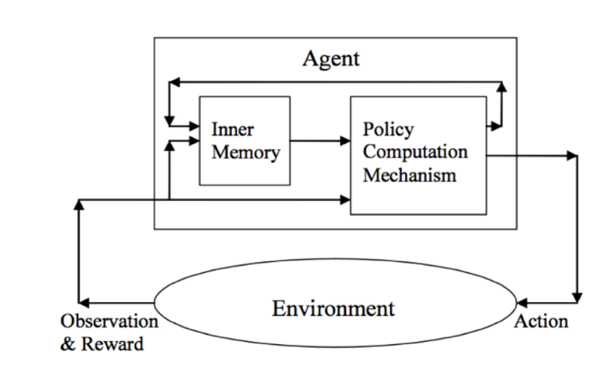
\includegraphics[width=0.45\textwidth]{agent_with_memory.png}
  \caption{The agent model that has internal memory}
  \label{fig:agent memory}
\end{figure}

The internal memory of an agent can comprise instances that record what it has
encountered at each time step. Nearest Sequence Memory (NSM) and Utile
Suffix Memory (USM) algorithms are based on the instances.


\subsection{Utile Suffix Memory Algorithm}

The interaction between the agent implementing USM and the environment is described by
$A, O, R$, which are finite set of actions, finite set of observations and a reward function.
Like other instance based algorithms, USM records each of its raw instances
\cite{mccallum1995instance}. At each time step $t$, the agent executes action
$a_t \in A$ to get a new instance, gets observation $o_{t+1} \in O$, and get a
instant reward $r_{t+1}$ according to $R$, which is determined by the environment.
That new instance is formulated as
\begin{equation}
  T_{t+1}= (T_t, a_t, o_{t+1}, r_{t+1}). \label{equ:instance}
\end{equation}
$T_{t+1}$ is $T_t$'s successor and, similarly, $T_{t-1}$ is $T_t$'s predecessor.
Normally, in an environment with goals for agent to reach, chains of instances-from
initial instance to instance reached goal-are built during the learning phase.

In order to find hidden states from those instances chains, USM creates a suffix tree,
whose leaves present the state space and store clustered instances. Each node of the tree
can thus be uniquely identified by the string of labels on the path from node to the root,
and the string is called the node’s suffix. An instance is always deposited into the
nodes whose suffix matches its observation and action context, or suffix. That is,
for an instance $T_i$, if its suffix $[..., o_{t-3}, a_{t-3}, o_{t-2}, a_{t-2}, o_{t-1}, a_{t-1}]$
matches the suffix of some node, it would be put into that node (see Figure~\ref{fig:suffix tree}).
The set of instances that a node contains is written as $I(s)$. The suffix tree leaf which
instance $T$ belongs to is written as $L(T)$. It is inevitable that the action layer and
the observation layer appears alternately when tree grows (see Figure~\ref{fig:suffix tree}).

\begin{figure}[b]
  \centering
    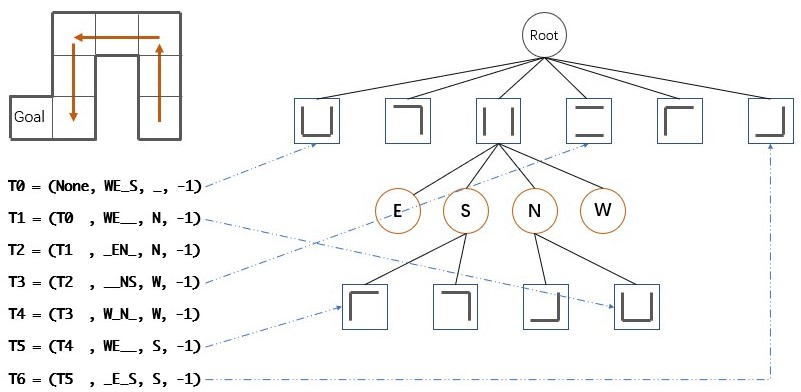
\includegraphics[width=0.45\textwidth]{usm_sample.jpg}
  \caption{The agent navigates itself in a maze (probably not the first time), generates
  a sequence of instances, and builds a suffix tree. The action layer and
  the observation layer appears alternately.}
  \label{fig:suffix tree}
\end{figure}

Besides the general nodes, there is another type of node called "fringe" node \cite{mccallum1995instance}.
The fringe nodes are actually the deepest layers of the suffix tree, however, we treated them
the inner instance buckets of the leaves previously mentioned. Fringe nodes also contain
instances according to the same suffix criterion used by non-fringe nodes. That is, 
if the suffix of a leaf is $[a_{t-2}, o_{t-1}, a_{t-1}]$, an 1-layer deeper fringe nodes of it
will stores the instance that matches suffix $[o_{t-2}, a_{t-2}, o_{t-1}, a_{t-1}]$. The agent decides
whether it should promote fringe nodes to leaves by Kolmogorov-Smirnov test, which determine the
instances in the fringes and that of their parent are drawn the same distribution.

The steps of USM is as below:

\begin{enumerate}
  \item The agent begins with a suffix tree that comprises a root node and an layer of
  observation nodes as leaves, i.e., the agent only acts according to its observation.

  \item The agent chooses an action according to $\epsilon$-greedy policy, executes it and
  generates an instance (see Equation ~\ref{equ:instance}).

  \item The agent insert the instance into the suffix tree. The instance is classified to
  leaves and fringes with the same suffix with that instance. 

  \item The agent triggers K-S test every $n$ additions of instance. If the Q-value of fringes
  and their parent are from different distributions, the fringes will be promoted to leaves.
  The instance will always be added to fringes and leaves that have the same suffix with the instance.
  Q-value table will be updated after every addition of instance. Time step increases and algorithm
  jumps to step 2.
\end{enumerate}

There are two obvious deficiencies of the USM algorithm. Firstly, in the USM algorithm,
the number of states may exponentially increase as the number of steps grows, but many
states are redundant, which correspond to the same state in the real environment. Thus, it
will reduce the efficiency of the algorithm. Secondly, since the initial Q value of all leaves
is initialized with 0, the $\epsilon$-greedy policy may lead to overfitting. Because
the $\epsilon$-greedy policy of USM treats the second best and the worst the same, it drastically
decrease the probability to explore other actions which may get higher reward. For example,
we found that in the first few steps, the agent may get negative default return after
choosing actions at some states, which decreases the probability of exploring those actions
when at those states again.

\section{Compressed Suffix Memory Algorithm}

In order to overcome the weaknesses of USM. We re-constructed the work flow of agent in maze
environments. Firstly, we introduces the blind exploration. Exploration and exploitation
is a key issue in reinforcement learning. Agent could first make a blind policy exploration
of the environment, obtaining some heuristic experience, and apply it to following reinforcement
learning. We found that the longest non-repetitive observations of the maze and the frequency
of goals can decently presents the local complexity and the scale of the environment, respectively.
The heuristic experience can be used to improve the algorithm:

\begin{enumerate}
  \item The depth of the suffix tree could be constrained. We tried to locate the redundant
  states of USM and found a potential cause. The suffix tree may grow so deep that a leaf's
  suffix is longer than most paths from start to goal. By deducing the length of most paths
  from start to goal as $l$ and limiting the suffix tree's depth to $2l$ can reduce the
  generation of less useful leaves. So we set $l$ as the sum of longest horizontal edge and
  vertical edge found by the blind search, since in most situations, paths generated by
  the best policy are shorter than $l$.

  \item Instances in tree node could be denser. Instead of doing K-S test every $n$ instances
  added, which may lead to overfitting at some leaves, agent only triggers K-S test when leaves
  and their fringe nodes are holding enough instances. The minimum number $b$ of instances to do K-S
  test is deduced from blind exploration, since $b$ should vary with environment scale. In practice,
  we find the frequency of goals in blind exploration well describes the environment scale.

  \item The $\epsilon$-greedy approach can be improved. The main problem of
  $\epsilon$-greedy approach is that it treats the second best and the worst the same, hence
  decreasing the probability to explore the second best action. We use boltzmann
  sampling to balance between exploration and exploitation, which assigns actions with similar
  Q value similar probabilities to encourage agent to explore or exploit them all, instead of
  only the best. The probability to choose an action $a_i$ at leaf $s$ with temperature $t$ is
    \begin{equation}
      p(s, a_i) = e(s, a_i)/ \sum_a{e(s, a)} \label{equ:boltzmann},
    \end{equation}  
  which $e$ is
    \begin{equation}
      e(s, a) = \exp( (Q(s, a) - \max Q(s))/t )
    \end{equation}

\end{enumerate}

The details and the pseudo code (see Algorithm~\ref{alg:CSM}) form of the CSM algorithm is as below.

\begin{enumerate}

  \item The agent begins with a suffix tree that comprises a root node and an layer of
  observation nodes as leaves, i.e., the agent only acts according to its observation.

  \item The agent randomly explores the environment for a number of times. The agent deduces the
  the effective path length $l$ to goal and minimum number $b$ of instances to do K-S test
  in that exploration. The maximum depth of the suffix tree is set to $2l$.

  \item The agent executes action and interacts with the environment at time step $t$.
  It records its learning history as an instance $T_t$ (see Equation~\ref{equ:instance}).
  For all $s$, no matter $s$ is leaf or fringe, if the suffix of $s$ matches the suffix of
  $T_t$. Their instance set are updated as:
    \begin{equation}
      I(s) \leftarrow I(s) \cup {T_t}.
    \end{equation}
  Let $L(T)$ be the leaf which instance $T$ belongs to. $L(T_t)$ is cached to agent memory.

  \item For each instance added, the agent does one Bellman iteration with the leaves of
  of the states:
    \begin{equation}
      Q(s,a) \leftarrow R(s,a)  + \gamma Pr(s'|s,a)U(s').
    \end{equation}
  Let $I(s,a)$ be the subset of $I(s)$ that contains all the instances that executed
  action $a$. $U(s')$ is the utility of the state $s'$, calculated as
  $U(s) = \max_{a \in A} Q(s,a)$. $R(s,a)$ and $Pr(s'|s,a)$ are the estimated immediate
  reward and the transition probability, respectively, that drawn from the instance chains:
    \begin{equation}
      R(s,a) = \frac{\sum_{T_i \in I(s,a)}r_i} {|I(s,a)|},
    \end{equation}

    \begin{equation}
      Pr(s'|s,a) = \frac{|\forall{T_i \in I(s,a) \ s.t. \ L(T_{i+1} = s')}|} {|I(s,a)|}.
    \end{equation}
  
  \item Agent perform Kolmogorov-Smirnov when $L(T_t)$ is not the same as $L(T_{t-1})$ and
  $L(T_t)$ holds enough instances (more than $b$). The expected discounted reward of instance
  $T_i$ is written as $H(T_i)$, and is defined as:
    \begin{equation}
      H(T_i) = r_i + \gamma U(L(T_{i+1}))
    \end{equation}
  Agent calculates every $Q(T_i)$ for instances of leaf and those of immediate fringe nodes,
  then determines whether they are from the same distribution. If they are not, those
  fringe nodes would be promoted as leaves.

  \item Agent does Boltzmann sampling to choose the next action, i.e., with
  probability $p(s, a_i)$ the agent chooses $a_i$ as $a_{t+1}$ (see Equation~\ref{equ:boltzmann}).
  In practice, we encourage agent to do random exploration for $n_r$ times, and then perform
  Boltzmann sampling method with descendant temperature.
  Time step increase to $t+1$ and algorithm jumps to step 3.
\end{enumerate}

\begin{algorithm}[h]
	\renewcommand{\algorithmicrequire}{\textbf{Input:}}
	\renewcommand{\algorithmicensure}{\textbf{Output:}}
	\caption{Compressed Suffix Algorithm}
	\label{alg:CSM}
	\begin{algorithmic}[1]
		\REQUIRE iteration steps $n$, radom steps in iteration $n_r$
		\ENSURE average discounted return $ADR$
    \STATE Initialize path length $l$, and minimum number $b$ of instance required to do K-S test
    by blind exploration
    \STATE Initialize temperature $t$ as positive infinity
    \STATE Initialize a suffix tree with depth limitation $2l$
    \STATE Initialize agent with random start position
		\FOR{$i=0$ to $n$}
		  \IF{$i>n_r$}
		    \STATE $t$ decreases from 0.5 to nearly 0 as $i$ increases
      \ENDIF

      \STATE Choose action $a$ by boltzmann sampling and execute it (see Equation~\ref{equ:boltzmann})
      \WHILE{not moved after executed $a$}
        \STATE Choose action $a$ by boltzmann sampling with higher $t$ and execute it
      \ENDWHILE

      \STATE Generate instance $T$ according to the execution of $a$ just now
      \STATE Insert $T$ into the suffix tree, and find the leaf node $s$ the instance belongs
      \STATE $I(s) = I(s) \cup {T_t}$
      \STATE $Q(s,a) = R(s,a) + \gamma Pr(s'|s,a)U(s')$
      \STATE $R(s,a) = {\sum_{T_i \in I(s,a)}r_i}/{|I(s,a)|}$
      \STATE $Pr(s'|s,a) = {|\forall{T_i \in I(s,a) \ s.t. \ L(T_{i+1} = s')}|} / {|I(s,a)|}$
      
      \IF {$|I(s)| > b$}
        \STATE do K-S test between $H(T)$s of $s$ and its fringe nodes, get p\_value $p$ 
        \IF {$p<0.1$}
          \STATE promote fringe nodes to leaves
        \ENDIF
      \ENDIF

      \IF {agent at goal}
        \STATE Initialize agent with random start position
      \ENDIF
    \ENDFOR
    \STATE Use boltzmann sampling at low temperature on $Q(s, a)$ to produce average
    discounted reward $ADR$ (see Equation~\ref{equ:adr})
		\STATE \textbf{return} $ADR$
	\end{algorithmic}  
\end{algorithm}

\section{Experiment}

\subsection{Experiment Setup}

We run algorithms with three well-known benchmarks: Tiger-Grid, Hallway and McCallum 
as well as a large Prim Maze generated by Prim algorithm randomly
(see ~Figure \ref{fig:mazes}). The characteristics of POMDP benchmarks are described
below (see ~Table \ref{table:benchmarks}), where $|S|$, $|A|$, $|\Omega|$, $r_d$, $r_p$, $r_g$, 
denotes the number of states, the number of actions, the number of observations, default
reward, penalty and goal, respectively. The $|A|$ is 4 because the action of the agent
normally includes: moving south, west, east and north. However, problems differ in some
details.

\begin{figure}[h]
  \centering
    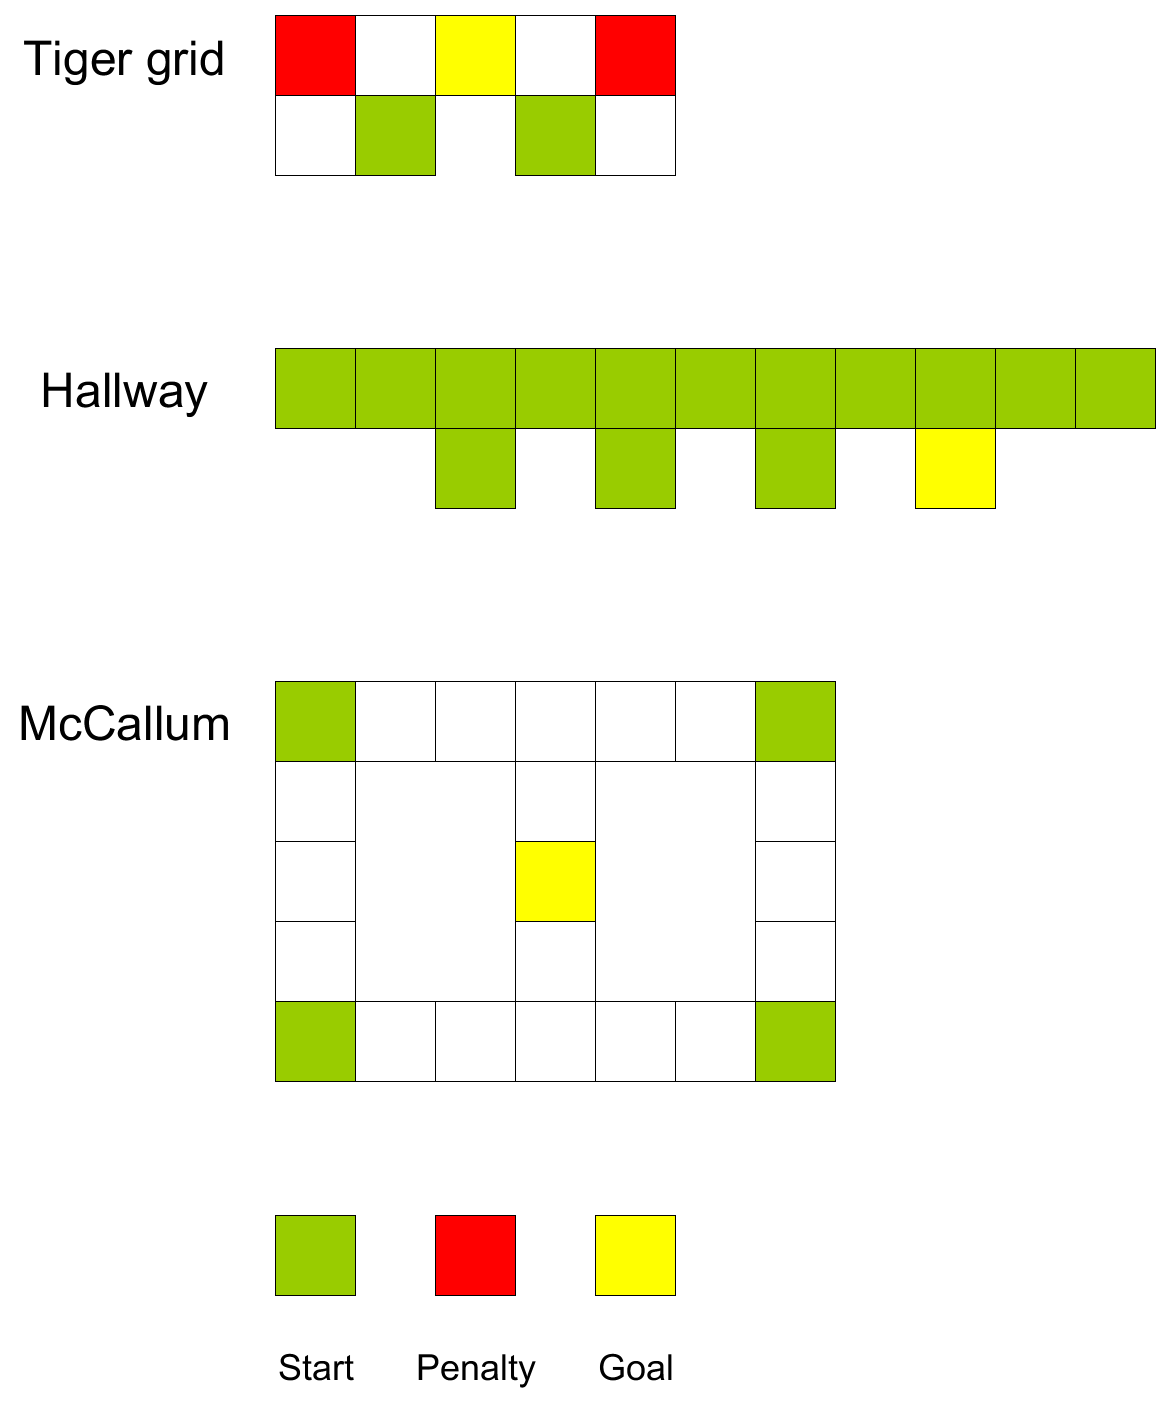
\includegraphics[width=0.45\textwidth]{mazes.png}
  \caption{Benchmark mazes}
  \label{fig:mazes}
\end{figure}

\begin{table}[h]
  \caption{Benchmarks}
  \label{table:benchmarks}
  \centering
  \begin{tabular}{lllllll}
    \toprule
    problem         & $|S|$          & $|A|$          & $|\Omega|$  &$r_d$  &$r_p$  &$r_g$\\
    \midrule
    Tiger-Grid      & 9              & 4              & 7           & -0.1  & -4    & 16  \\
    Hallway         & 15             & 4              & 4           & -0.1  &     & 32  \\
    McCallum        & 23             & 4              & 9           & -0.1  &     & 18  \\
    Prim Maze       & 154            & 4              & 16          & -0.1  &    & 96  \\
    \bottomrule
  \end{tabular}
\end{table}

In Tiger-Grid, the agents are initially assigned to one of two definite starting positions.
The probability of each starting position is 0.5. The goal of the model is to make the agent
reach the goal position as soon as possible. Once the agent reaches the goal position,
it will be reset to two starting positions. Tiger-Grid's maze comprises two penalty positions
where agent will receive a negative reward. 

In Hallway, similar to Tiger-Grid problem but still different, agent will be reset randomly
to a non-goal state. The Hallway does not include any penalty position. Furthermore, the hallway
adds 4 landmarks as hint for agent to discover hidden states.

In McCallum, after reached the goal, the agent will be randomly reset at one of the 4 corners.
There are 3 south-north hallways, which are deliberately designed for agent to distinguish, since
they are ambiguous. 

In Prim Maze, which is randomly generated by Prim algorithm and mean to be big. $|S|$ of Prim Maze
is several times the $S$ of others. When the agent arrives at the goal, Prim Maze will reset
the agent to a random state in the maze.

We evaluate average discounted reward, $ADR$, in the experiment:
\begin{equation}
  ADR = \frac{\sum_{i=0}^{n_{trails}} \sum_{j=0}^{n_{steps}} \gamma^j r^j}{n_{trails}}, \label{equ:adr}
\end{equation}
$ADR$ is widely considered to be a good evaluation of the quality of a value function. The higher
the $ADR$ is, the more intelligent the agent is considered to be. We track the changing of $ADR$ through time
to determine whether CSM helps the agent to learn faster and better.
  
Our experiment uses a discount factor $\gamma=0.9$, an exploration probability $\epsilon=0.1$ for USM.
The boundary value of the Kolmogorov-Smirnov test is $p=0.1$. We iterate the USM, CSM and random algorithm
2048 times, and set check points per 48 iteration. In each check point we test our model 256 times
within 96 steps, i.e., $n_{trial}$ is 256 (see Equation~\ref{equ:adr}) in $ADR$ calculation.

\subsection{Experiment Results}

%The experiment results of CSM, USM and random algorithm are shown in  Table \ref{table:results} and Figure  \ref{fig:tiger_grid_result} to \ref{fig:prim_maze_result}. It should be noted that due to the randomness of the ADR measurement method, the results of ADR may fluctuate. Therefore, the max ADR in Table \ref{table:results}  represents the ADR when the algorithm results start to stabilize, rather than the maximum value of the experimental ADR results.
%(see Figure~
%\ref{fig:tiger_grid_result}, \ref{fig:agent_duration_step}).
The experiment results of CSM, USM and random algorithm are shown below (see Figure~\ref{fig:agent_adr_time}).
It should be noted that even if $n_trail$-set to 256-seems large enough, the results of $ADR$ may still fluctuate.
Therefore, we record (plateau $ADR$, time) tuples in the table below (see Table \ref{table:results}), when $ADR$ starts to become relatively stationary, rather than when $ADR$ gets maximum. 

\begin{figure}[!ht]
	\centering
	\subfloat[Tiger Grid]{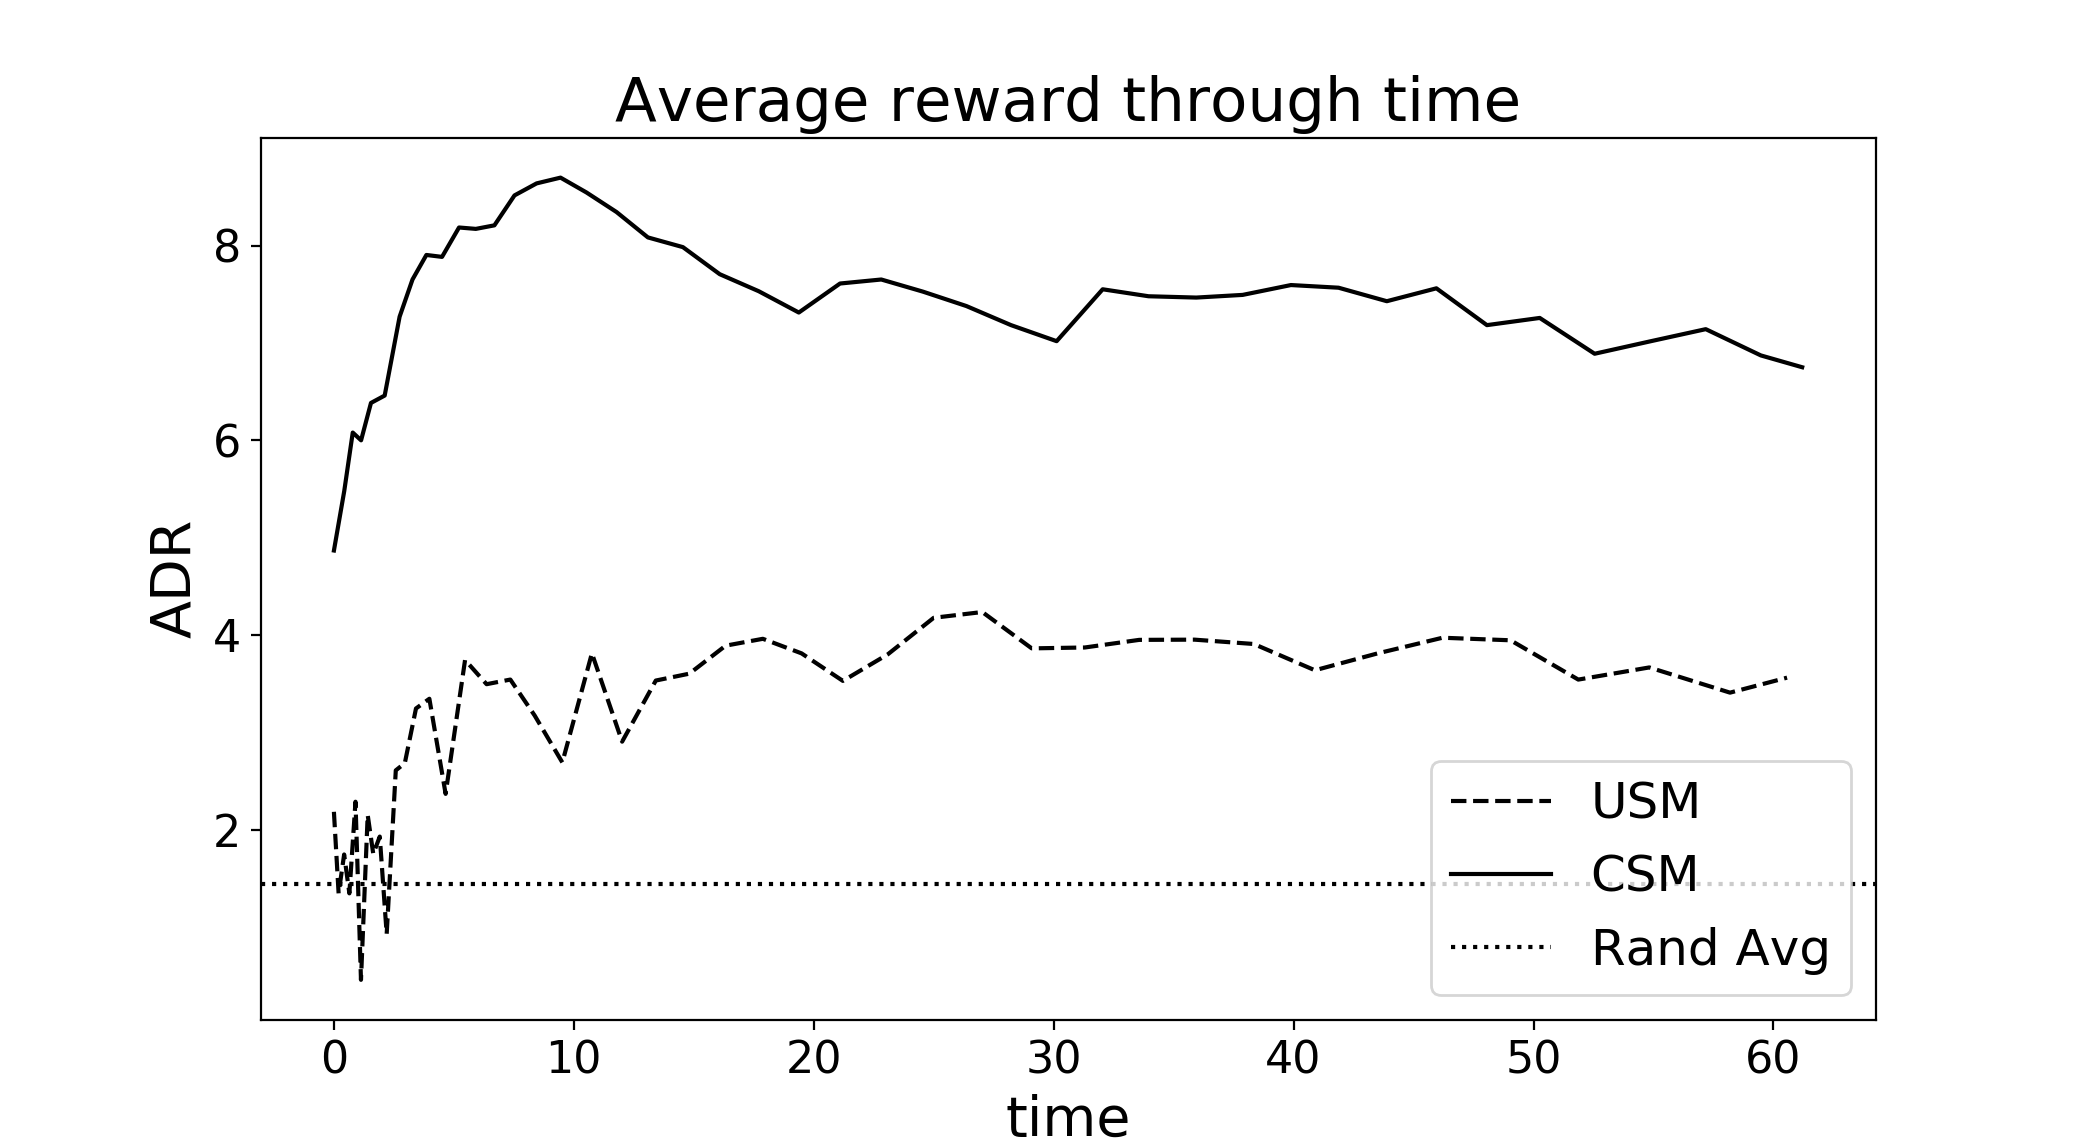
\includegraphics[width=2.8in]{06-13-21-48/tiger_grid_result.png}}\\
 \subfloat[Hallway]{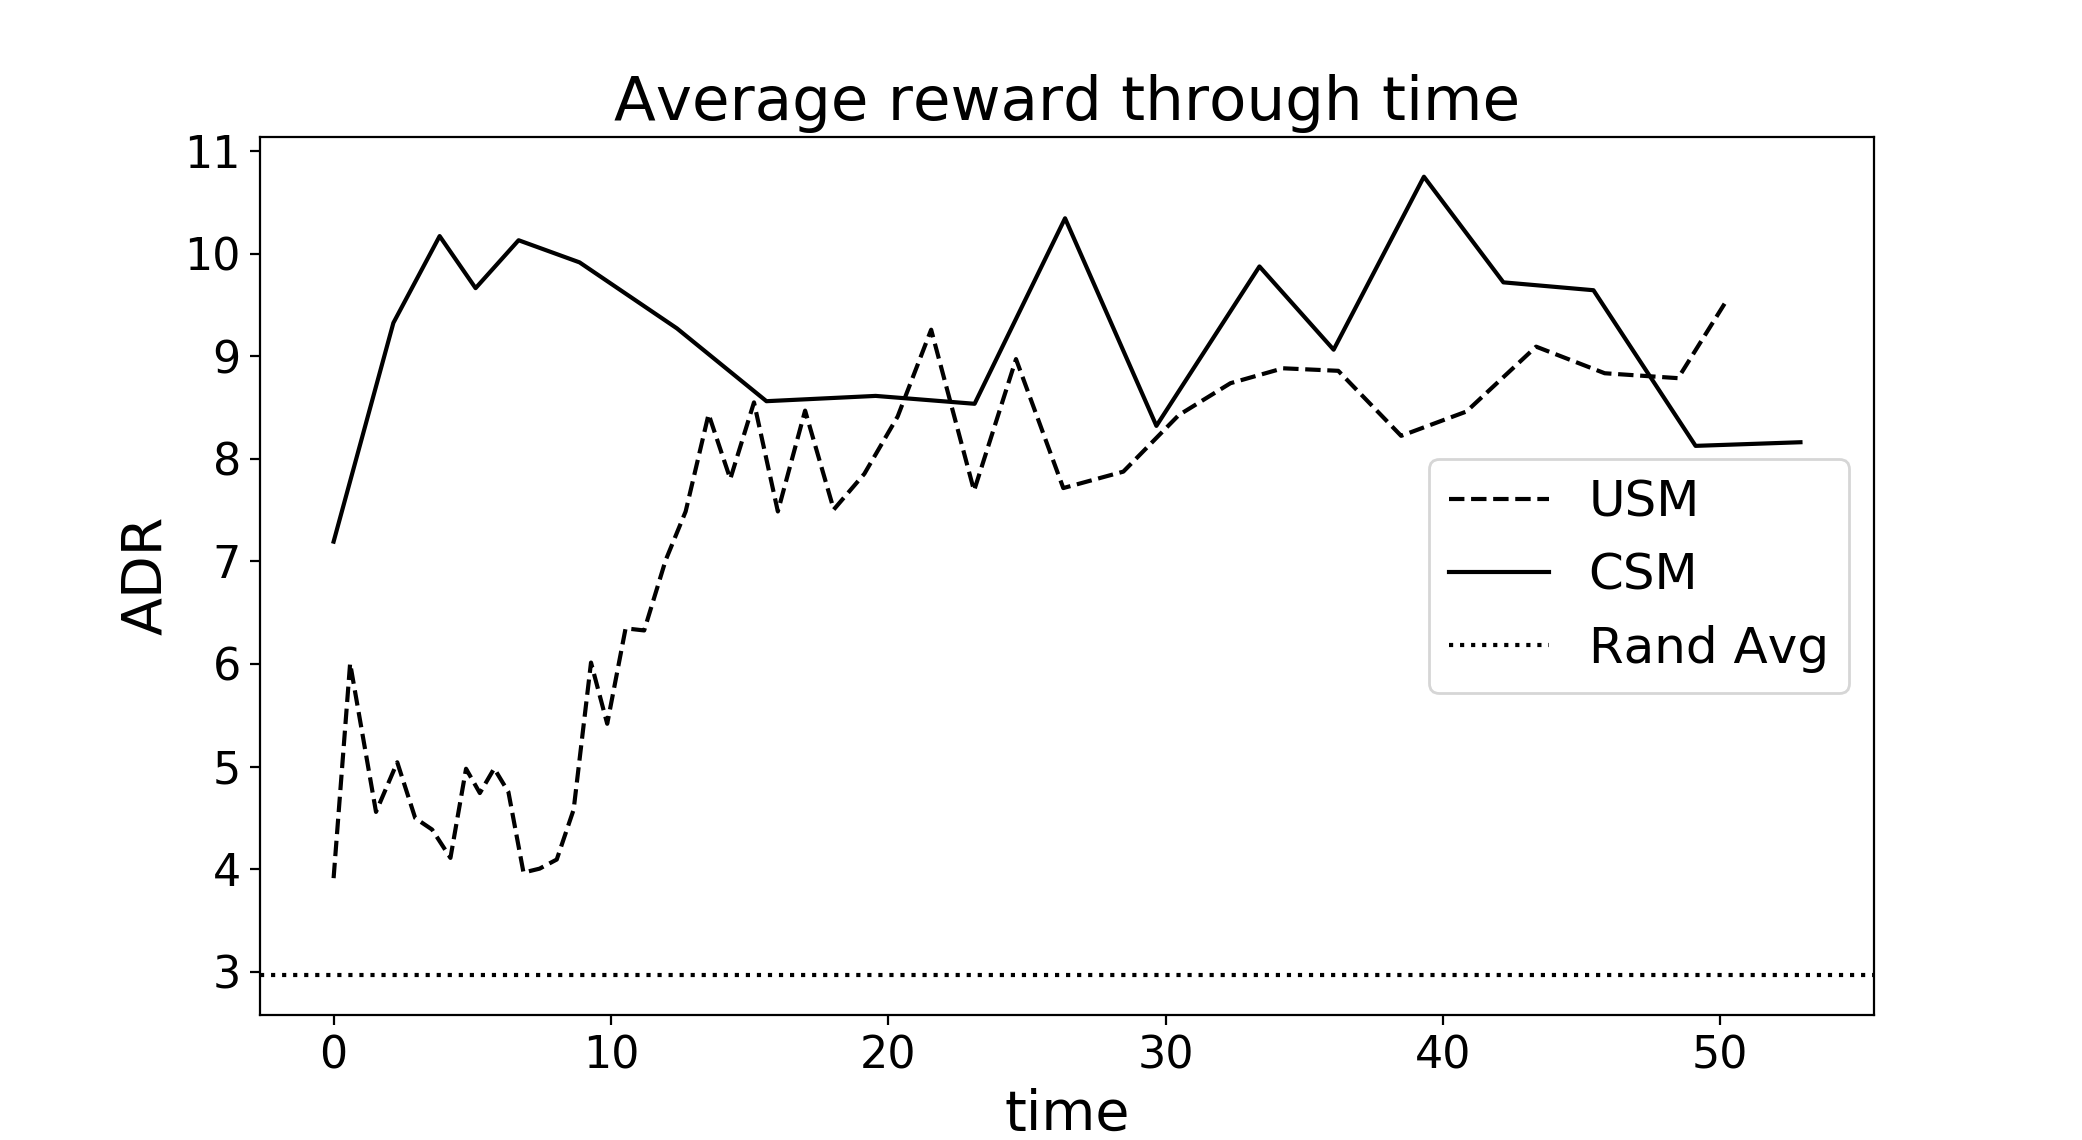
\includegraphics[width=2.8in]{06-13-21-48/hallway_result.png}}\\
 \subfloat[McCallum]{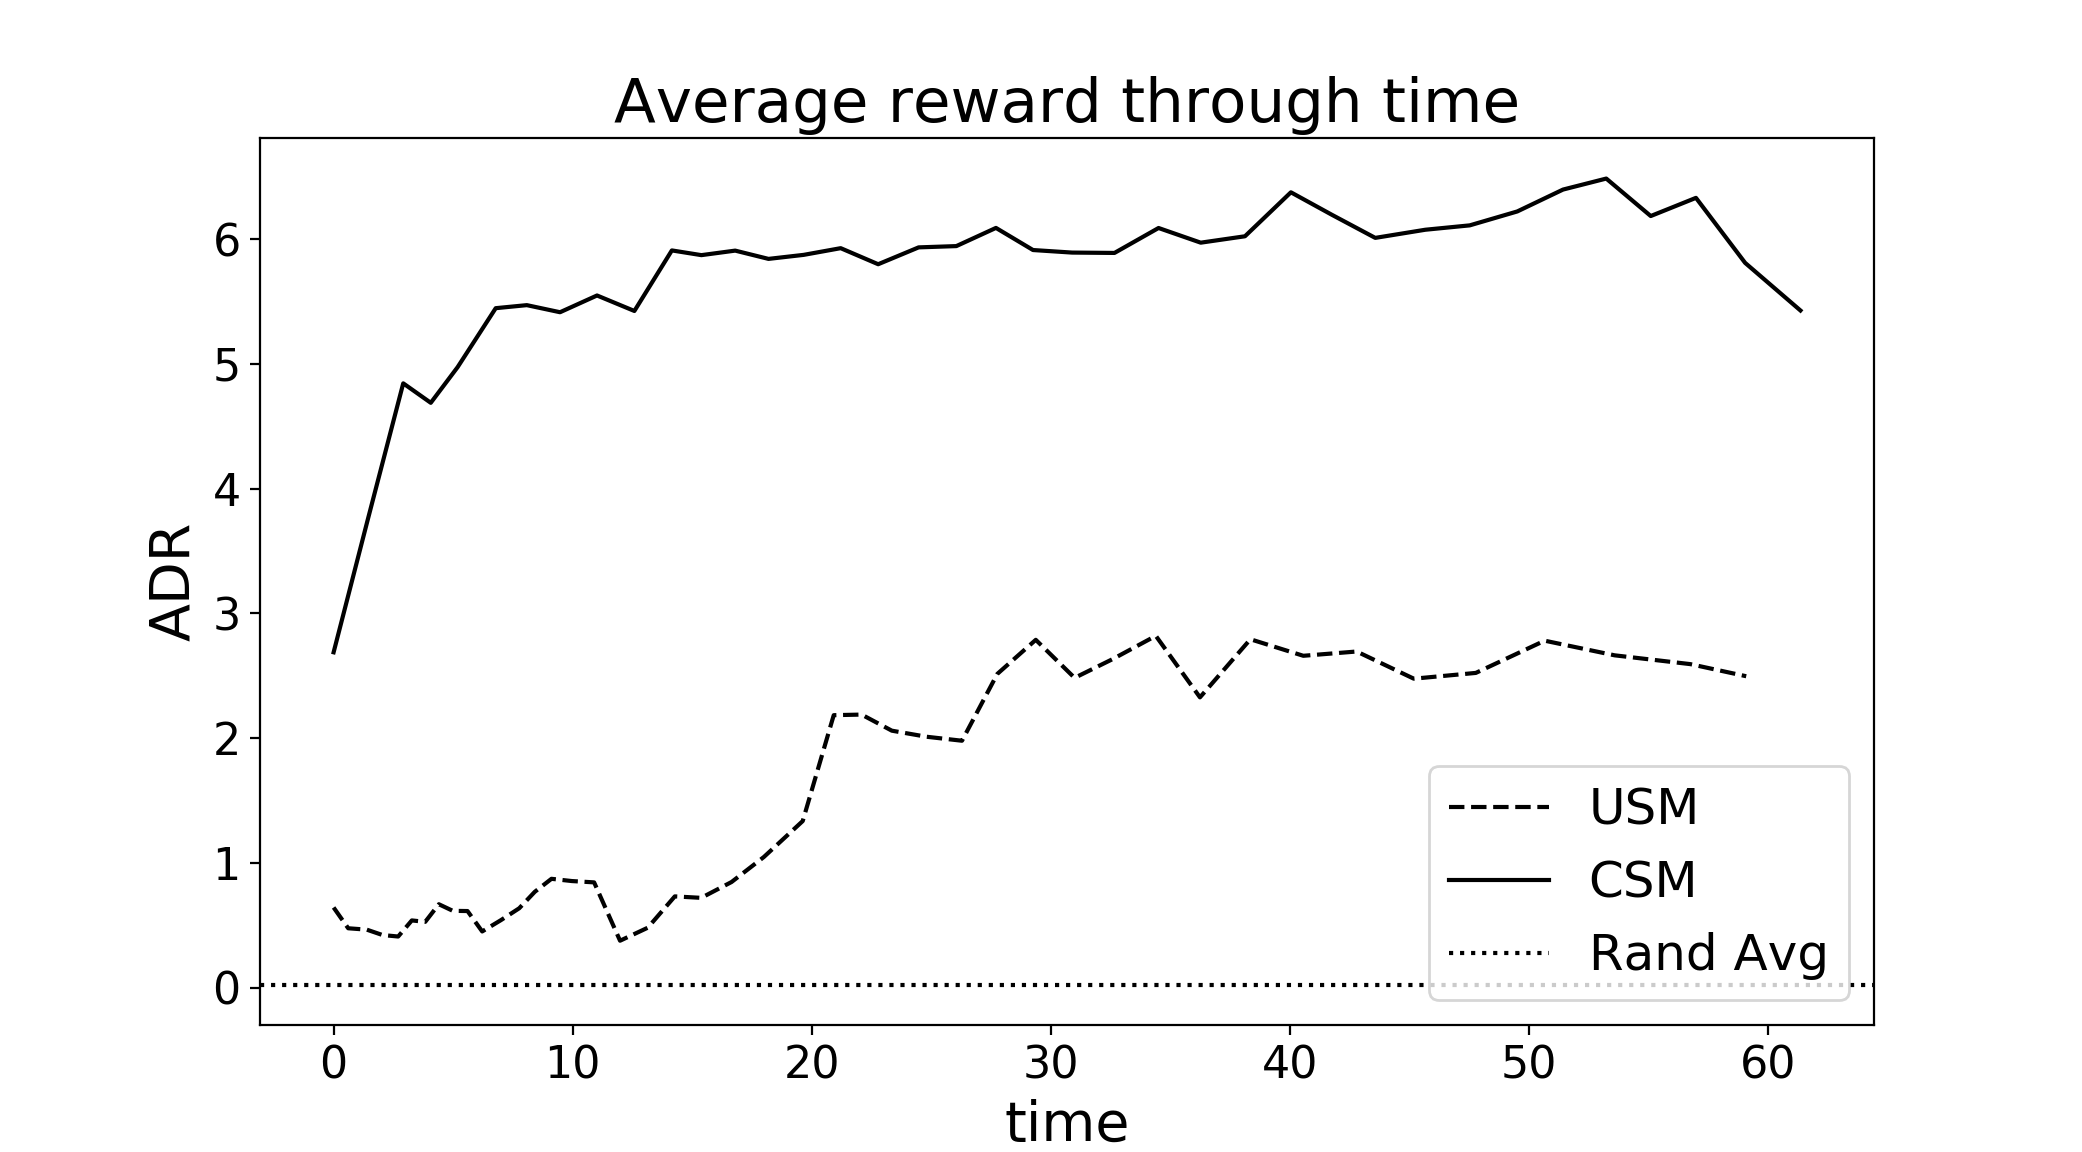
\includegraphics[width=2.8in]{06-13-21-48/mccallum_result.png}}\\
 \subfloat[Prim Maze]{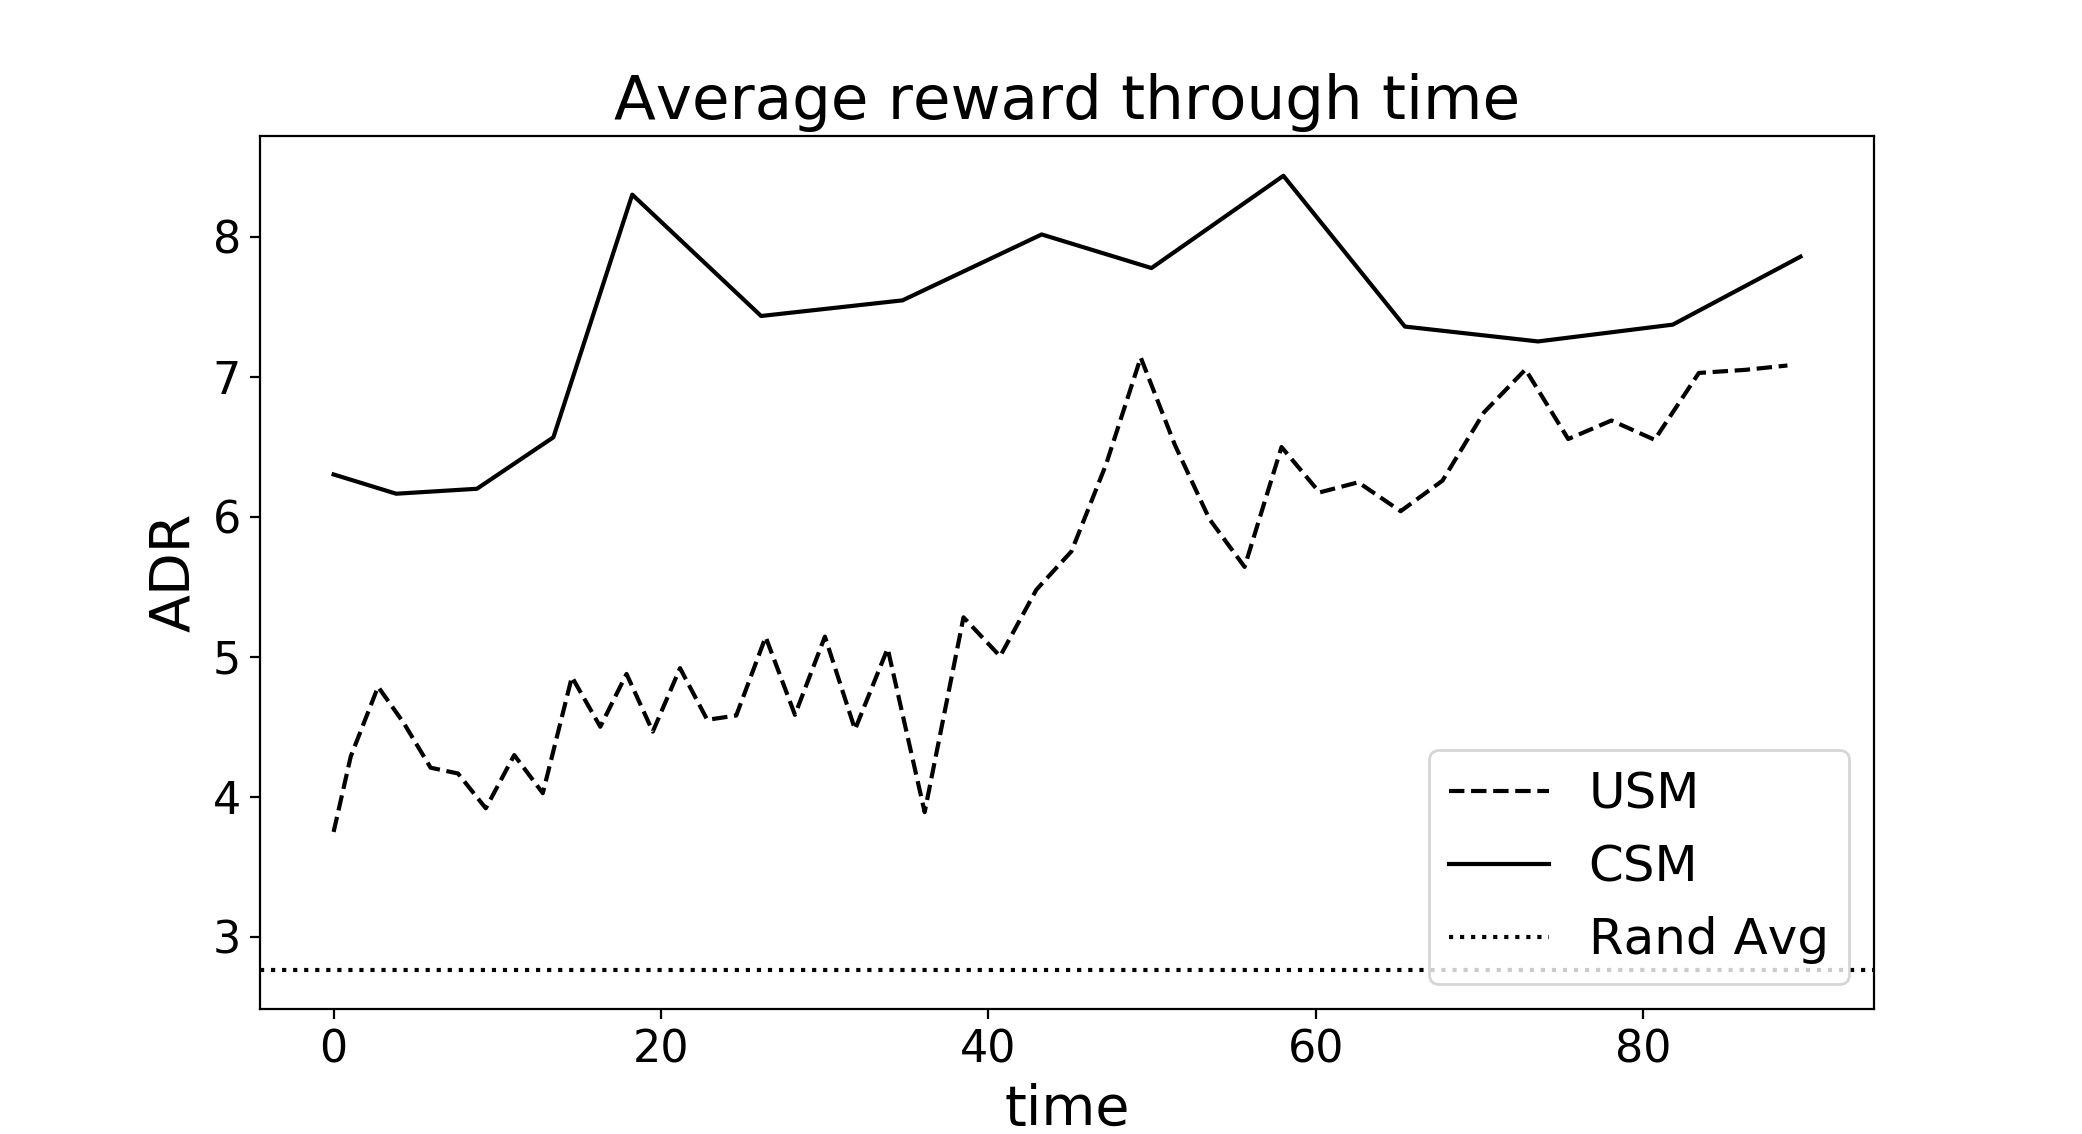
\includegraphics[width=2.8in]{06-13-21-48/prim_maze_result.png}}\\
 \caption{Performance of different agent on different benchmarks; y-axis is $ADR$,
 x-axis is runtime in seconds.}
 \label{fig:agent_adr_time}
\end{figure}

\begin{table}[h]
	\caption{Experiment Results}
	\label{table:results}
	\centering
	\begin{tabular}{lcccc}
		\toprule
                  &\multicolumn{2}{c}{plateau $ADR$}      &\multicolumn{2}{c}{time taken} \\ 
                  \cmidrule(r){2-3}                 \cmidrule(r){4-5}
    problems      & USM         & CSM               &USM           & CSM      \\
    \midrule
		Tiger-Grid    & 3.81        & 8.70              & 10.75        & 9.45     \\ 
		Hallway       & 8.43        & 10.13             & 13.52        & 6.67     \\ 
		McCallum      & 2.82        & 5.90              & 34.39        & 14.15    \\ 
    Prim Maze     & 7.13        & 8.30              & 49.30        & 18.24    \\ 
    \bottomrule
	\end{tabular}
\end{table}

\subsection{Experiment Results Analysis}

% On the Tiger-Grid problem, the CSM algorithm quickly reached a very high ADR in a short
% time after the start of the experiment, and as the experiment progressed, the ADR of the
% CSM was basically stable at around 8. In contrast, the experimental results of the USM
% algorithm have large fluctuations in the early stage of the experiment, and the
% experimental results in the latter part of the experiment are basically stable at 4, which
% is only half of the CSM.

% On the Hallway problem, the experimental ADR results of both algorithms showed large fluctuations, 
% and they had very similar stable maximum ADR. However, from the time point of view, the CSM 
% algorithm reaches the stable maximum ADR running time is only half of the USM, that is, the CSM 
% has twice the processing speed of the USM on the Hallway problem.



% On the McCallum Maze problem, similar to the performance in the Tiger-Grid
% problem, the CSM algorithm quickly reached a very high ADR in the short time after
% the start of the experiment, and as the experiment progressed, the ADR of the CSM
% was basically stable at 6. In contrast, the experimental results of the USM algorithm
% did not increase significantly in the early stage of the experiment, and only showed
% a growth trend in the later stage of the experiment. Despite this, USM's final ADR
% is only about 3, far less than CSM. This shows that in the case of McCallum Maze problem, 
% CSM can explore the whole problem and find the optimal strategy more quickly and better than USM.

% On large dataset problems, such as the Prim Maze problem in the experiment, CSM can also perform 
% faster and better than USM. From the experimental results, the CSM achieved a stable maximum ADR 8 
% in about 20 seconds, while the USM had an ADR of less than 5 in the same time. Even in the mid-term 
% of the experiment, USM has experienced rapid growth, but its time cost is almost three times that of 
% CSM, and ADR is still lower than CSM.

% In addition, it can be seen from the experimental results that at the beginning of the experiment, although both algorithms have not gained experience through learning, CSM has obtained a higher ADR than USM. This can be explained in two ways.
% First, because the CSM algorithm uses the Boltzmann algorithm to explore, the agent does not perform only the optimal action at the stage of exploitation like the USM does, but other non-optimal actions have a certain probability to be executed.
% Secondly, because CSM uses a strategy of not going back to go forward bolder, when it does not fall into a dead end.
% It is for these two reasons that CSM is able to explore the full maze and discover the goal faster than the USM, thus obtaining a higher ADR.

In Tiger-Grid, CSM algorithm quickly reached a very high $ADR$ in a short
time after the start of the experiment. As the experiment progressed, the $ADR$ of
CSM algorithm converged to 7.5. In contrast, the $ADR$ of USM algorithm fluctuated
drastically in the early stage of the experiment, and became stable at around 4, which
was only half of the CSM algorithm.

In Hallway, the $ADR$ of both algorithms fluctuated violently,  
and converged to a similar value. However, when comparing time taken to reach those,
CSM algorithm reached plateau $ADR$ taken the half runtime of USM algorithm, i.e.,
the agent adopted CSM algorithm have learned twice as fast as agent adopted USM algorithm
in Hallway.

In McCallum, similar to the performance in Tiger-Grid, CSM algorithm quickly reached
a very high $ADR$ in short time after the start of the experiment. As the experiment
progressed, the $ADR$ of CSM algorithm was basically stable at 6. On the other hand,
the $ADR$ of USM algorithm have not significantly increased in the early stage. What's more,
USM algorithm got a far less max $ADR$ than CSM algorithm, which is only about 3. The figure
indicated that in McCallum, CSM algorithm could find a better policy more quickly than USM
algorithm.

In larger scale problems, such as the Prim Maze, CSM algorithm also performed
faster and better than USM. From the experiment results, CSM algorithm achieved a plateau
$ADR$ about 8 in about 20 seconds. USM algorithm, meanwhile, only reached around 5.
Even if in the mid-stage of the experiment, where the $ADR$ of USM has experienced arapid growth,
its time cost was almost three times that of CSM, and had a still lower $ADR$.

In addition, it can be seen from the experiment result that at the beginning of the experiment,
although both algorithms have not gained experience through learning, CSM has obtained a higher
$ADR$ than USM. This can be explained in two ways:
\begin{enumerate}
  \item CSM algorithm uses the Boltzmann sampling method to choose action, the agent does
  not only perform the best action at the stage of exploitation, but  other non-optimal actions,
  which resist overfitting at early stage.
  
  \item CSM rises the $temperature$ of Boltzmann sampling when agent continously bumps into walls,
  which helps agent get out of that position. That ensures the efficiency of exploration.
  
\end{enumerate}
It is for these two reasons that CSM algorithm is able to understand the environment better and
discover the goal faster than USM algorithm, hence obtaining a higher $ADR$.

Overall, It can be seen that CSM algorithm helps agent to learn faster and better than USM algorithm


\section{Conclusion}



%In this paper, the USM algorithm is described in detail, and the defects of USM
%algorithm are proposed. Based on the original algorithm, some suggestions for improvement
%are proposed. Then the CSM (Compressed Suffix Memory) algorithm is proposed. At the end of
%this paper, the content of the maze experiment is introduced to test the CSM algorithm, and
%compared with the results of the USM algorithm, it shows that the CSM algorithm does have
%some improvement effects.

%In this paper, we briefly described the POMDP model and the USM algorithm, and pointed out the 
%shortcomings of USM. For the original USM algorithm, we proposed optimization suggestions in 
%three aspects, constraint of the depth of the suffix tree, densification of instances in tree node, and 
%utilization of boltzmann sampling, respectively, and introduced a new CSM algorithm. 
%Finally, the experiments of four benchmark problems we implemented also confirmed that the improvements 
%of the CSM algorithm are indeed effective to boost efficiency. 

%Although the result of experiment improves greatly, there are still some problems to be consider. 
%For example, the boltzmann sampling will increase the computational cost of the algorithm, thereby increasing the time of each iteration.
%And how to maximize the use of experience, that agents have learned, to the future exploration is also a problem.


In this paper, POMDP model and instance-based approach USM algorithm are described firstly. 
Then this paper introduced a new CSM algorithm based on the original USM algorithm, improving it in three aspects,  constraint of the depth of the suffix tree, densification of instances in tree node, and 
utilization of boltzmann sampling. 
The experiment results confirmed that both effect and efficiency are promoted comparing CSM to USM. 

%Although the result of experiment improves greatly, there are still some problems to be consider. 
%For example, the boltzmann sampling will increase the computational cost of the algorithm, thereby increasing the time of each iteration.
%And how to maximize the use of experience, that agents have learned, to the future exploration is also a problem. For example, the boltzmann sampling costs extra computational resources of the algorithm, thereby increasing the time of each iteration.


Although experiment results demonstrate great improvement, 
there are still some problems to be consider. For example, the boltzmann sampling costs extra computational resources of the algorithm, thereby increasing the time of each iteration.
Furthermore,how agent mines more effective heuristic standards based on the acquired exploration experience is our future research direction. 




% References
\clearpage
\small
\bibliographystyle{named}
\bibliography{dai_2019}


\end{document}
